%\documentclass[11pt,a4paper]{article}
%\usepackage{fullpage}
%\usepackage{beamerarticle}
%\documentclass[handout,xcolor=pdftex,dvipsnames,table]{beamer}
\documentclass[hyperref={unicode=true}]{beamer}

%\usepackage{pgfpages} 
%\pgfpagesuselayout{resize}[a4paper,border shrink=5mm,landscape] 

\usepackage[utf8]{inputenc}
\usepackage[russian]{babel}
\usepackage{../clrscode3e} 
%\usepackage[all]{xy}
\usepackage{colortbl}
%\usepackage{xcolor}
\usepackage{pstricks, pst-tree, pst-node}
\usepackage{epsfig}
\usepackage{multicol}
\usepackage{array}
\usepackage{wrapfig}
%\usepackage{listings}

\definecolor{orange}{cmyk}{0,0.52,1,0}

%\usepackage{beamerthemesplit}
\psset{levelsep=1cm, treesep=1cm, linewidth=0.5pt, levelsep=30pt} 
\newcommand{\tnd}[1]{\Tcircle{\makebox[5mm][c]{#1}}} 

\AtBeginSection[]
{
  \begin{frame}<beamer>{Раздел}
    \tableofcontents[currentsection]
  \end{frame}
}


\AtBeginSubsection[]
{
  \begin{frame}<beamer>{Раздел}
    \tableofcontents[currentsection,currentsubsection]
  \end{frame}
}


\newtheorem{rtheorem}{Теорема} 
\newtheorem{rdefinition}{Определение} 
\newtheorem{rconsequence}{Следствие} 
%default}
%themesplit}

\title{Сжатие текстов}
\subtitle{Дискретный анализ 2012/13}
\author{Андрей Калинин, Татьяна Романова}
\date{27 апреля 2013\,г.}
\usetheme{default}
%\usefonttheme{serif}
\usefonttheme[onlymath]{serif}
%\usefonttheme{professionalfonts}
%\usetheme{default} 


\begin{document}

\frame{\titlepage}

\frame
{
  \frametitle{Литература}


  \begin{itemize}
  \item Witten, Moffat, Bell, Managing gigabytes: compressing and
    indexing documents and images.
  \item M.\,J.\,Attalah, Algorithms and Theory of Computation Handbook, 12.3 Dynamic Huffman Coding.
  \item Ватолин Д., Ратушняк А., Смирнов М., Юкин В., Методы сжатия
    данных. Устройство архиваторов, сжатие изображений и видео. 
  \item Сэлмон Д., Сжатие изображений и звука, М.:Техносфера, 2006. 
  \end{itemize}
}

\section{Коды Хаффмана}

\frame{
  \frametitle{Неоднозначность алгоритма Хаффмана}
  \begin{itemize}
  \item Правое и левое поддерево может кодироваться 1-0 или 0-1. 
  \item В случае, если есть несколько символов с одинаковыми
    частотами, нет правила по их однозначному выбору. 
  \end{itemize}
  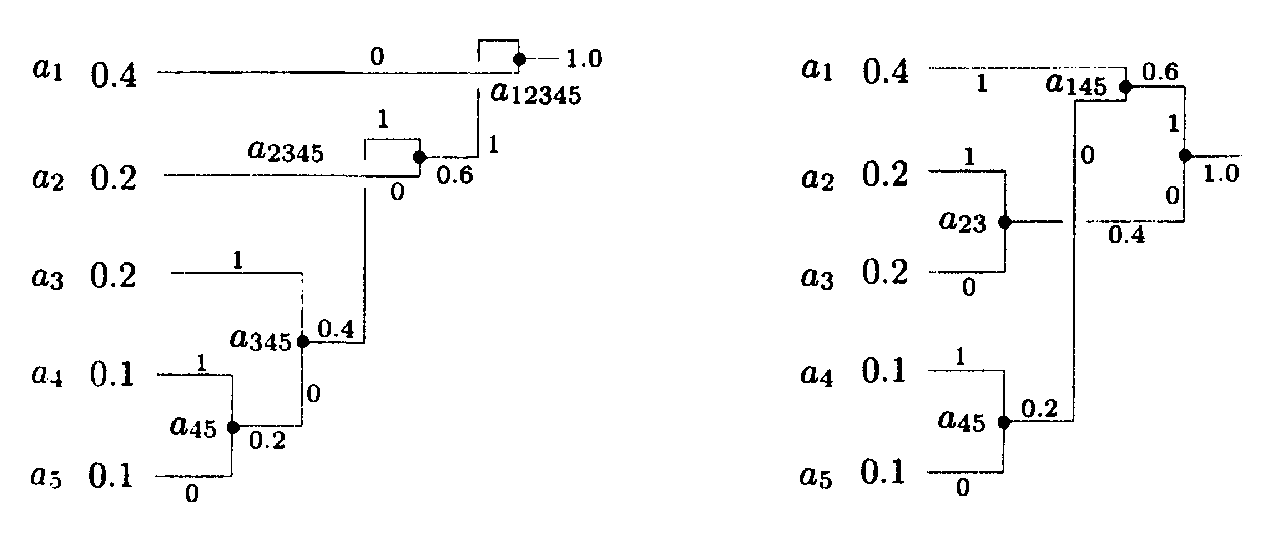
\includegraphics[width=\textwidth]{huffman-1.eps}
}

\frame{
  \frametitle{Ограниченность кодирования Хаффмана}
  \begin{itemize}
  \item Данные с равновероятными символвами не сжимаются. 
  \item Однако, не все строки, в которых частоты символов
    равновероятны --- случайны. 
  \item Напрмер, последовательность 
\[
a_1a_1\ldots a_1a_2a_2\ldots a_2a_3a_3\ldots
\]
где каждый символ встречается длинными сериями одинаковой длины ---
может быть сжата методом RLE (run-length encoding), но не методом
Хаффмана. 
\item Для двухсимвольного алфавита код Хаффмана будет $\langle 0, 1
  \rangle$ вне зависимости от частот символов.
\item Декодер должен получить от кодера статистику использования
  символов (что увеличивает объём) или кодер с декодером должны
  использовать статический набор частот (что ухудшает компрессию). 
  \end{itemize}
}


\subsection{Адаптивное кодирование}

\frame{
  \frametitle{Основная идея}
  \begin{itemize}
    \item Кодер и декодер начинают с пустого дерева, которое
      модифицируется по ходу работы. 
    \item Первый входной символ записываеся в выходной файл в несжатой
      форме и помещается в дерево с частотой 1, ему присваивается
      код. 
    \item В следующий раз он будет закодирован с использованием
      кода, соответствующего его расположению в дереве, а
      соответствующий счётчик увеличен на 1. 
    \item Аналогичная операция проделывается со следующий символом. 
    \item При добавлении символа в дерево или изменении частот может потребоваться
      перестроить дерево.
  \end{itemize}
}

\frame{
  \frametitle{Специальный символ ESC}
  \begin{itemize}
    \item Нужно отличать закодированные символы от их первого
      появления в прямом коде. 
    \item Для этого вводится дополнительный символ, ESC (Escape),
      который предваряет первое появление символа. 
    \item Этот символ всегда есть в дереве и имеет частоту 1, 
          при появлении новых символов код escape-символа удлинняется.
  \end{itemize}
}

\frame{
  \frametitle{Модификация дерева Хаффмана}
   Любое построенное стандартным алгоритмом дерево Хаффмана c $n$ листьями можно представить 
   в виде последовательности $x_0, x_1,..., x_{2n-2}$ такой, что
  \begin{enumerate}
    \item Веса (частоты), записанные в узлах составят невозрастающую последовательность:
    $$
      weight(x_0) \ge weight(x_1) \ge ... \ge weight(x_{2n-2})
    $$
    \item Для любого элемента $i$ ($0 \le i \le n - 2$) элементы на позициях $2i + 1$ и $2i+2$ являются его сыновьями. 
  \end{enumerate}
}

\frame{
  \frametitle{Кодирование. Описание.}
  \begin{itemize}
    \item Дерево Хаффмана хранится в массиве (аналогично куче из пирамидальной сортировки).
    \item Изначально в дереве находится только ESC-символ.
          Он всегда будет самым правым элементом массива.
    \item Если нужно добавить новый узел, на место ESC-символа помещается новый родитель,
          новый узел становится левым сыном, ESC~--- правым.
    \item У узла, соответствующего считанному символу, счетчик частоты увеличивается на 1.
    \item Также на 1 нужно увеличить счетчики всех предков. При этом частоты узлов в массиве могут перестать
         быть невозрастающей последовательностью. Тогда нужно "переподвесить" текущий нарушающий порядок 
         узел (и его поддерево) на место узла, хранящегося в самом левом элементe массива с меньшей частотой.
  \end{itemize}
}

\psset{treesep=1.5cm, levelsep=16pt}

\frame
{
  \frametitle{Кодирование. Пример.}
  1. Кодируем строку ABBCD. Начальное дерево:

  \pstree {\tnd{1,Es}} 


  2. Считываем A, выводим 0100 0001 (код 'A'), обновляем дерево:

  \pstree {\tnd{2}}{\tnd{1,A} \tnd{1,Es}}
  

  3. Считываем B, выводим 1 (Esc) и 0100 0010 (код 'B'), обновляем дерево:
  
  \pstree {\tnd{2}}{\tnd{1,A} 
                    \pstree{ \tnd{2}} {\tnd{1,B} \tnd{1,Es}}}
  ~$\Rightarrow$
  \pstree {\tnd{3}}{ \pstree{ \tnd{2}} {\tnd{1,B} \tnd{1,Es}}
                     \tnd{1,A}}
}

\frame
{
  \frametitle{Кодирование. Пример.}
  4. Считываем В, выводим 00, обновляем дерево:

  \pstree {\tnd{4}}{ \pstree{ \tnd{2}} {\tnd{1,A} \tnd{1,Es}}
                     \tnd{2,B}}

  5. Считываем C, выводим 01 (Esc) и 0100 0011 (код 'C'):
  \pstree {\tnd{5}}{ \pstree{ \tnd{3}} {\pstree{ \tnd{2}} {\tnd{1,C} \tnd{1,Es}} \tnd{1,A}}
                     \tnd{2,B}}


  6. Считываем D, выводим 001 (Esc) и 0100 0100 (код 'D'):
   \pstree {\tnd{6}}{ \pstree{ \tnd{4}} {\pstree{\tnd{2}} {\tnd{1,C} \tnd{1,A}}
                                         \pstree{\tnd{2}} {\tnd{1,D} \tnd{1,Es}}}
                     \tnd{2,B}}


}

\frame {
   \frametitle{Кодирование. Реализация. }
  \begin{codebox}
   \Procname{$\proc{DH-Init}$}
  \li $root \gets 0$
  \li $child(root) \gets UNDEFINED$
  \li $parend(root) \gets UNDEFINED$
  \li $weight(root) \gets 1$
  \li \For each letter $a$ in $Alphabet$ \Do
  \li $leaf[a] \gets UNDEFINED$ \End
  \li $leaf[ESC] \gets root$ \End
  \end{codebox}

}

\frame {
   \frametitle{Кодирование. Реализация. }
  \begin{codebox}
   \Procname{$\proc{DH-Encoding}$}
  \li $\proc{DH-Init}$
  \li \While not $eof(fin)$ and next symbol is $a$ \Do
  \li $\proc{DH-Encode-Symbol}(a, fout)$
  \li $\proc{DH-Update}(a)$ \End
  \end{codebox}
}

\frame {
   \frametitle{Кодирование. Реализация. }
  При поиске кода мы поднимаемся по дереву, поэтому нужен стек. Заметим, что все левые сыновья имеют нечетные номера, правые - четные.
  \begin{codebox}
   \Procname{$\proc{DH-Encode-Symbol}(a,fout)$}
  \li $S \gets$ empty stack
  \li $n \gets leaf[a]$
  \li \If $n = UNDEFINED$ \Then 
  \li     $n \gets leaf[ESC]$ \End
  \li \While $n != root$ \Do
  \li    \If $n$ нечетное \Then
  \li      $\proc{Push}(S, 1)$
  \li      \Else $\proc{Push}(S, 0)$ \End
  \li    $n \gets parent(n)$ \End
  \li $\proc{Send}(S, fout)$
  \li \If $leaf[a] = UNDEFINED$ \Then
  \li    пишем в $fout$ 8-битный код 
  \li    $\proc{DH-Add-Node}(a)$ \End
  \end{codebox}
}

\frame {
  \frametitle{Кодирование. Реализация. }
  \begin{codebox}
   \Procname{$\proc{DH-Add-Node}(a)$}
  \li $leaf[ESC]$ становится внутренним узлом с весом 1, 
  \li его левый сын $leaf[a]$ с весом 0,
  \li правый - $leaf[ESC]$ с весом 1.
  \end{codebox}
}

\frame {
  \frametitle{Кодирование. Реализация. }
  \begin{codebox}
   \Procname{$\proc{DH-Update}(a)$}
   \li $n \gets leaf[a]$
   \li \While $n != root$ \Do
   \li    $weight(n) = weight(n) + 1$
   \li    Поиск самого левого соседа, с которым можно поменяться
   \li    Иллюстрация: 6-й шаг примера
   \li    $m \gets n$
   \li    \While $weight(m-1) < weight(n)$ \Do
   \li        $m \gets m - 1$ \End
   \li    $\proc{DH-Swap-Nodes}(m, n)$
   \li    $n \gets parent(m)$ \End
   \li $weight(root) = weight(root) + 1$
  \end{codebox}
}


\subsection{Канонические коды Хаффмана}

\frame{
  \frametitle{Неоднозначность кодов Хаффмана}
  \begin{tabular}{lllll}
    \hline
    Буква & Частота & Код 1 & Код 2 & Код 3 \\
    \hline
    a & 10 & 000 & 111 & 000 \\
    b & 11 & 001 & 110 & 001 \\
    c & 12 & 100 & 011 & 010 \\
    d & 13 & 101 & 010 & 011 \\
    e & 22 & 01 & 10 & 10 \\
    f & 23 & 11 & 00 & 11 \\
    \hline
  \end{tabular}
}

\frame[plain]{
  \frametitle{Пример канонического кода}
  \begin{tabular}{lrl}
    100 & 17 & 00000000000000000 \\
    101 & 17 & 00000000000000001 \\
    102 & 17 & 00000000000000010 \\
    \ldots & \ldots & \ldots\\
    zepyhyr & 17 & 00001101010101000 \\
    zigzag & 17 & 00001101010101001 \\
    11th & 16 & 0000110101010101 \\
    120 & 16 & 0000110101010110 \\
    \ldots & \ldots & \ldots \\
    you & 7 & 1100001 \\
    I & 6 & 110001 \\
    in & 6 & 110010 \\
    was & 6 & 110011 \\
    a & 5 & 11010 \\
    and & 5 & 11011 \\
    of & 5 & 11100 \\
    to & 5 & 11101 \\
  \end{tabular}
}

\frame{
  \frametitle{Канонический код Хаффмана}
  \begin{itemize}
  \item Длины кодов для символов (слов) рассчитаны классическим
    способом. 
  \item Коды назначются по порядку. 
  \item Все слова в группе кодов одной длины сортируются в
    лексикографическом порядке. 
  \item Первый код в группе равен коду последнего слова в предыдущей
    группе без последнего бита и увеличенный на~1. 
  \item Имеет смысл для алфавитов больших размеров (слов)
  \item Позволяет не хранить дерево в явном виде. 
  \end{itemize}
}

\frame{
  \frametitle{Алгоритм построения канонического кода}
  \begin{codebox}
  \li \For $l \gets 1$ \To $maxlength$ \Do
  \li $numl[l] \gets 0$ \End
  \li \For $i \gets 1$ \To $n$ \Do
  \li $numl[l_i] \gets numl[l_i]+1$ \End
  \li $firstcode[maxlength] \gets 0$
  \li \For $l \gets maxlength-1$ \Downto $1$ \Do
  \li $firstcode[l] \gets (firstcode[l+1]+numl[l+1])/2$ \End
  \li \For $l\gets 1$ \To $maxlength$ \Do
  \li $nextcode[l] \gets firstcode[l]$ \End
  \li \For $i\gets 1$ \To $n$ \Do
  \li $codeword[i] \gets nextcode[l_i]$
  \li $symbol[l_i, nextcode[l_i]-firstcode[l_i]] \gets i$
  \li $nextcode[l_i] \gets nextcode[l_i]+1$ \End
  \end{codebox}
}

\frame{
  \frametitle{Построение канонического кода}
  \begin{tabular}{ccclccccc}
    \hline $i$ & $l_i$ & $codeword[i]$ & биты & 1 & 2 & 3 & 4 & 5 \\
    \hline
    1 & 2 & 1 & 01 & 0 & 1 \\
    2 & 5 & 0 & 00000 & 0 & 0 & 0 & 0 & 0 \\
    3 & 5 & 1 & 00001 & 0 & 0 & 0 & 0 & 1 \\
    4 & 3 & 1 & 001 & 0 & 0 & 1 \\
    5 & 2 & 2 & 10 & 1 & 2 \\
    6 & 5 & 2 & 00010 & 0 & 0 & 0 & 1 & 2 \\
    7 & 5 & 3 & 00011 & 0 & 0 & 0 & 1 & 3 \\
    8 & 2 & 3 & 11 & 1 & 3 \\
      &   &   & ~~~~~~$numl[l]$ & 0 & 3 & 1 & 0 & 4 \\
      &   &   & $firstcode[l]$ & 2 & 1 & 1 & 2 & 0 \\
      \hline
  \end{tabular} 
}

\frame{
  \frametitle{Деокдирование канонического кода Хаффмана}
  \begin{codebox}
    \li $v \gets \proc{Next-Input-Bit}()$
    \li $l \gets 1$
    \li \While $v < firstcode[l]$ \Do
    \li $v \gets 2v + \proc{Next-Input-Bit}()$
    \li $l \gets l+1$ \End
    \li \Return $symbol[l, v-firstcode[l]]$
  \end{codebox}
}

\frame{
  \frametitle{Вычисление длин кодов Хаффмана}
  \begin{enumerate}
  \item Создать массив $A$ из $2n$ элементов, прочитать в нижнюю
    половину частоты, в верхнюю половину поместить <<указатели>> на
    эти частоты. 
  \item Построить из верхней половины массива $A$ <<пирамиду>> (по
    значениям, соответствующим указателям). 
  \item Пройти по пирамиде, выбирая последовательно два минимальных
    элемента и помещая в пирамиду элемент с суммой значений
    выбранных. Заменять значения в удалённых элементах на номер
    родителя. 
  \item Восстановить по пирамиде из <<указателей>> на родителя длины
    кодов для каждого символа. 
  \end{enumerate}
}

\frame[plain]{
  \frametitle{Алгоритм вычисления длин кодов}
  \begin{codebox}
  \li \Comment Создать $A$ из $2n$ элементов. 
  \li \For $i \gets 1$ \To $n$ \Do
  \li $A[n+i] \gets c_i$, $A[i] \gets n+i$ \End
  \li $h \gets n$ 
  \zi \Comment Построить <<пирамиду>> из $A[1\ldots h]$,
  \zi \Comment В $A[1]$ хранится $m_1=\arg \min \{A[n+1]\ldots 2n\}$
  \li \While $h>1$ \Do 
  \li $m_1 \gets A[1]$, $A[1]\gets A[h]$, $h \gets h-1$
  \li \Comment Просеять <<пирамиду>> $A[1\ldots h]$ от $A[1]$
  \li $m_2 \gets A[1]$
  \li $A[h+1] \gets A[m_1]+A[m_2]$, $A[1]\gets h+1$
  \li $A[m_1] \gets A[m_2] \gets h+1$
  \li \Comment Просеять пирамиду $A[1\ldots h]$ от $A[1]$ \End
  \li $A[2] \gets 0$
  \li \For $i \gets 3$ \To $2n$ \Do
  \li $A[i] \gets A[A[i]]+1$ \End
  \end{codebox}
}

\frame[plain]{
  \frametitle{Этапы работы алгоритма}
  \begin{center}
  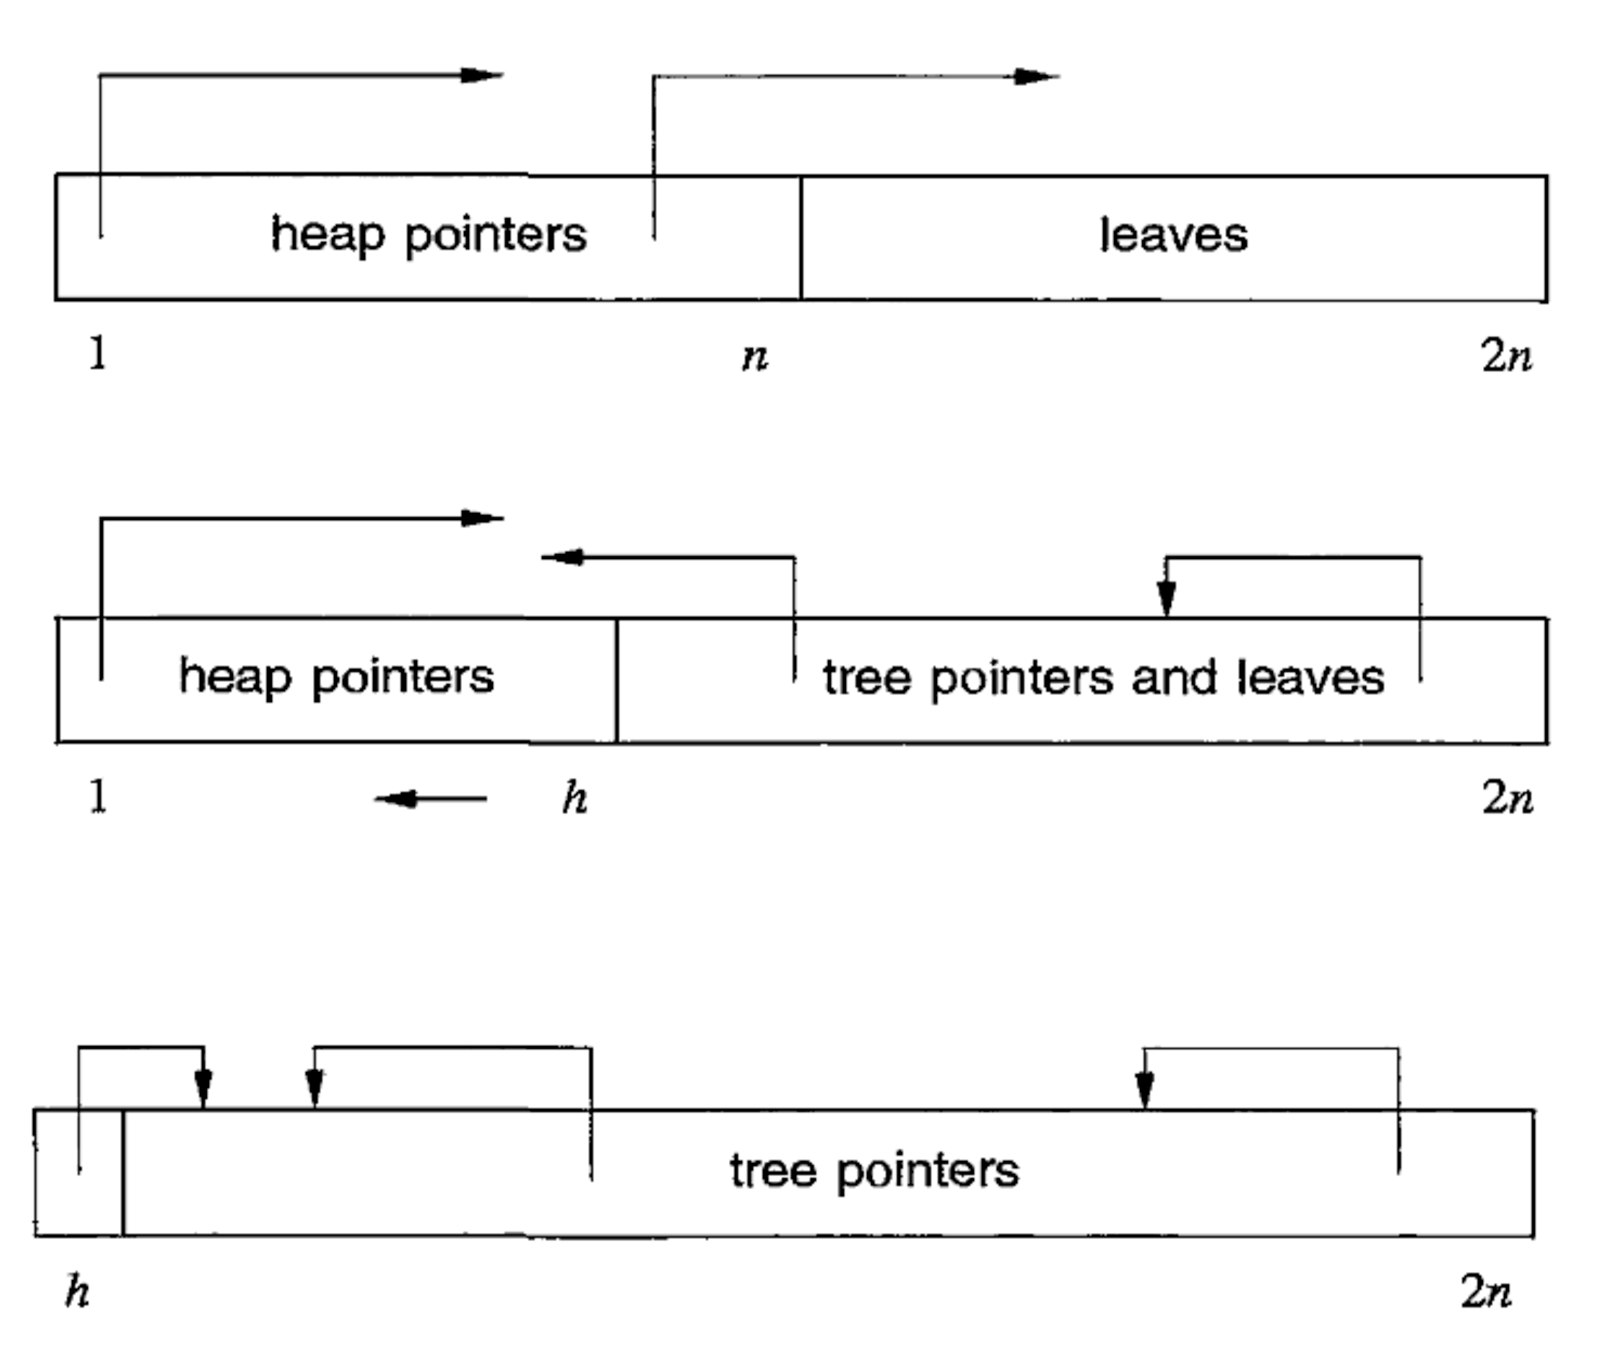
\includegraphics[height=.9\textheight]{gen-huf-code-length.eps}
  \end{center}
}

\frame[plain]{
  \frametitle{Извлечение минимальных частот}
  \begin{center}
  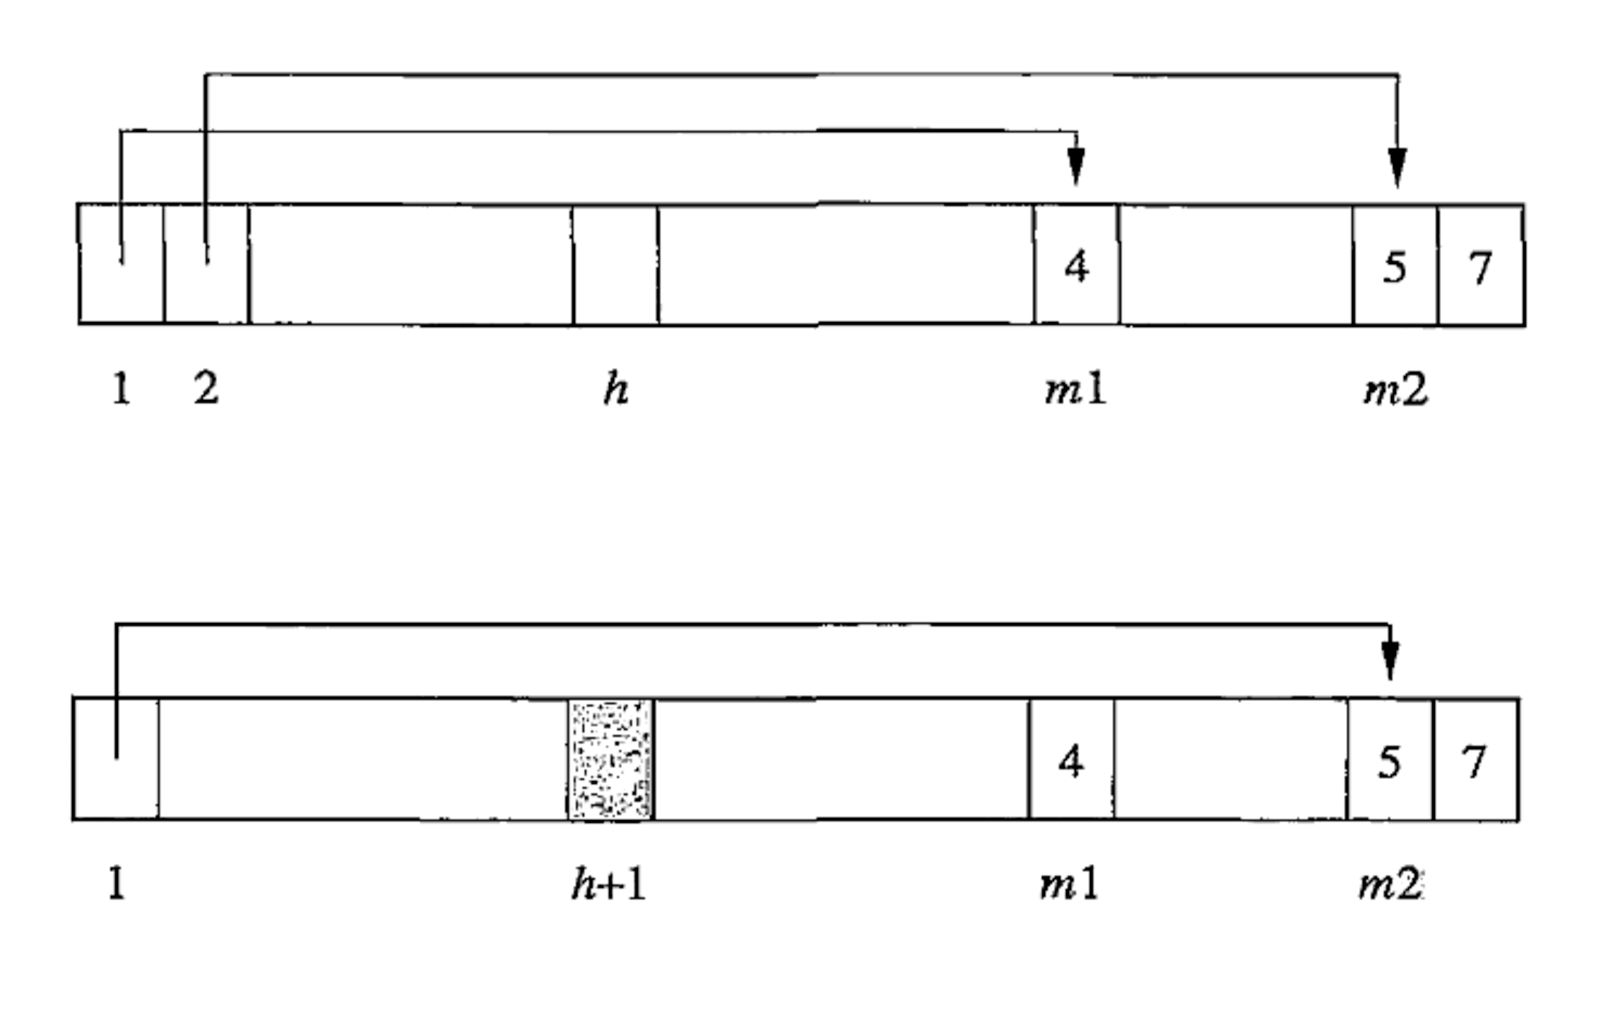
\includegraphics[width=\textwidth]{hc-heap-1.eps}
  \end{center}
}

\frame[plain]{
  \frametitle{Сохранение нового узла дерева}
  \begin{center}
  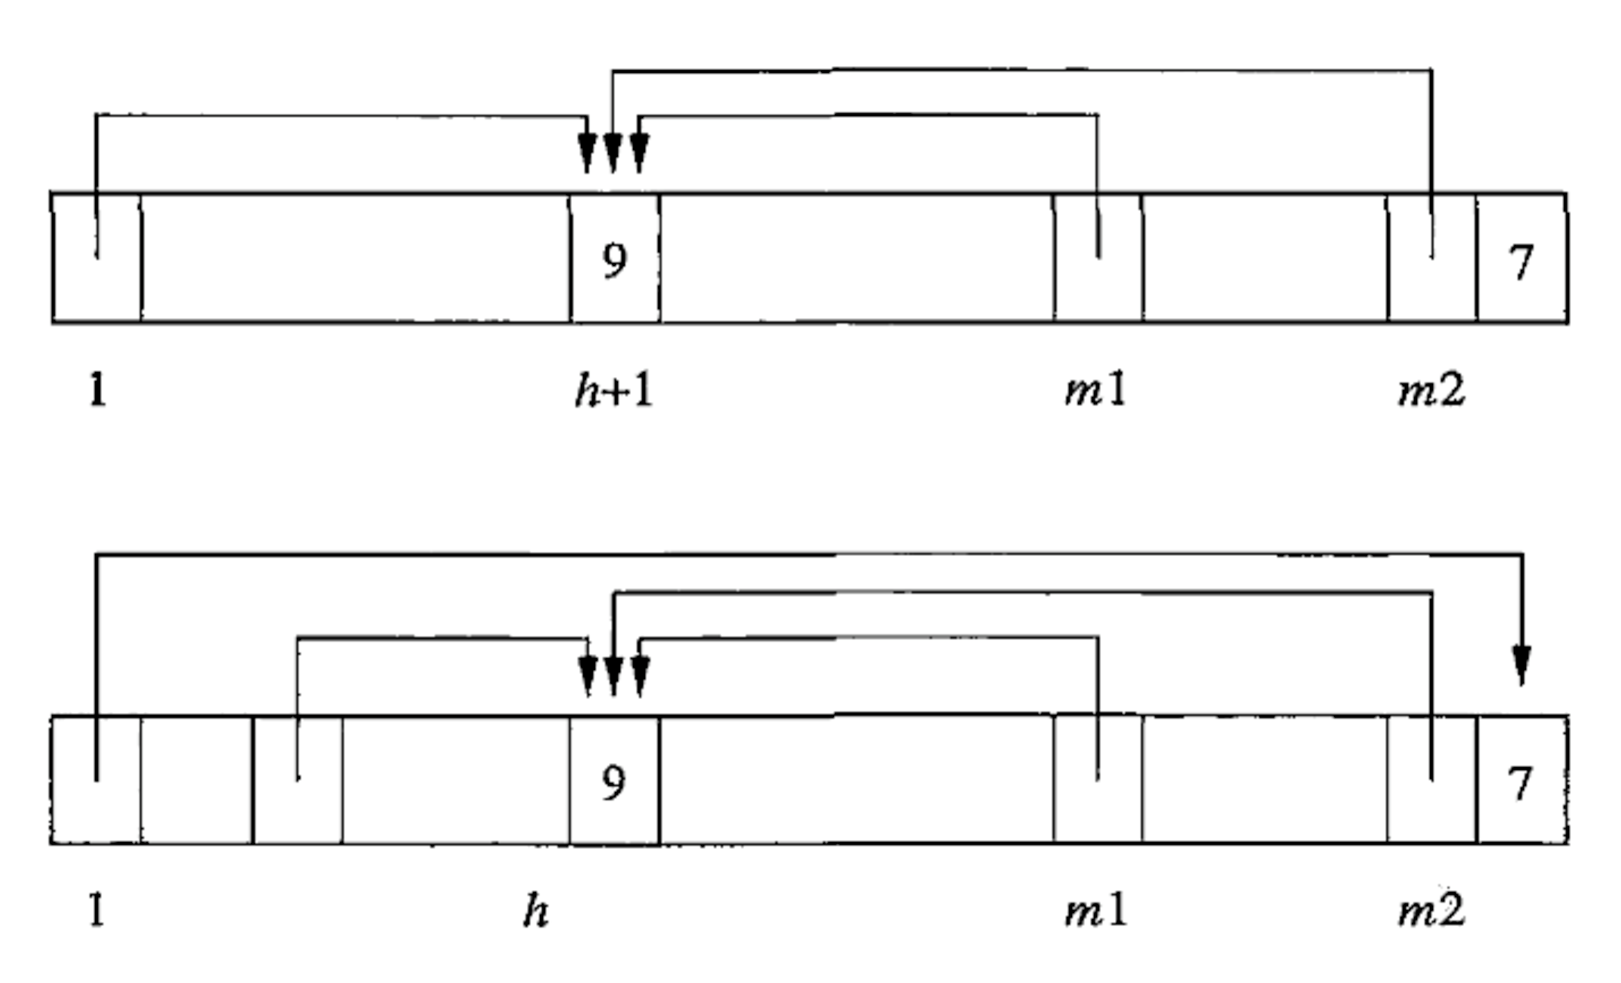
\includegraphics[width=\textwidth]{hc-heap-2.eps}
  \end{center}
}

\frame[plain]{
  \frametitle{Вычисление длин кодов}
  \begin{center}
  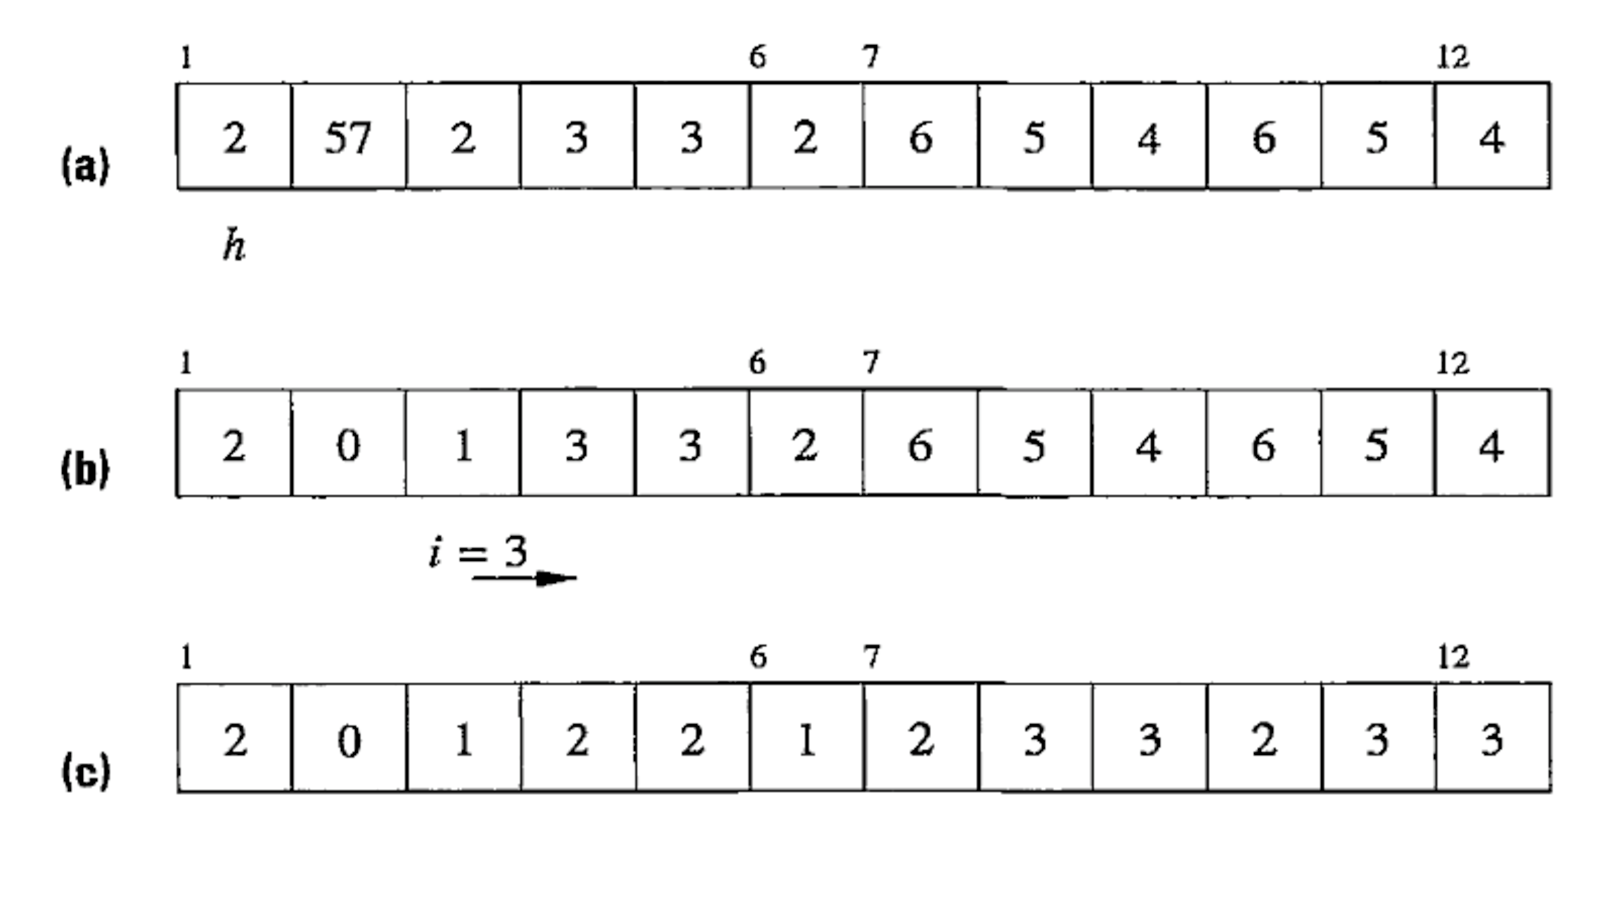
\includegraphics[width=\textwidth]{hc-heap-3.eps}
  \end{center}
}

\end{document}

